%%%%%%%%%%%%%%%%%%%%%%%%%%%%%%%%%%%%%%%%%%%%%%%%%%%%%%%%%%%%%%%%%%%%%%%%%%%%%%
% % % % % % %
%  Packages %
% % % % % % %

%---Base packages
\documentclass[a4paper,12pt,oneside]{report}	% document type (article, report, book)
\usepackage[utf8]{inputenc}			% encoding
\usepackage[T1]{fontenc}			% accent
\usepackage{lmodern}				% latin font
\usepackage{appendix}				% to be able to use appendices
\usepackage{tabularray}

%---Language(s)
\usepackage[english,frenchb]{babel}	% last language = typography by default
\addto\captionsfrench{				% to change the french names of...}
	\renewcommand{\appendixpagename}{Annexes}	% (default Appendices)
	\renewcommand{\appendixtocname}{Annexes}	% (default Appendices)
	\renewcommand{\tablename}{\textsc{Tableau}}	% (default \textsc{Table})
}

%---Page layout
%------> margins
	% 1st option -> geometry package
		%\usepackage[a4paper]{geometry}		% default parameters for A4
		%\usepackage[top=2in, bottom=1.5in, left=1in, right=1in]{geometry}
	% 2nd option -> a4wide package
		\usepackage{a4wide}		% A4 with smaller margins (the one I've chosen)
	% 3rd option -> fullpage package
		%\usepackage{fullpage}
%------> chapter style
	% 1st option -> fncychap package
		%\usepackage[style]{fncychap}		% style = Lenny, Bjornstrup, Sonny, Conny
	% 2nd option -> customized styles
		%
%------> cover page (UMONS template)
	\usepackage[fpms]{umons-coverpage}		% NEED "umons-coverpage.sty" file
	\umonsAuthor{Noms des auteurs : \\ Théau \textsc{Pauwels}
                                    \\ Mathys \textsc{Rogge}}
	\umonsTitle{Rapport de projet - Théorie des circuits}
	\umonsSubtitle{Synthèse d'un amplificateur de classe D}
	\umonsDocumentType{}
	\umonsSupervisor{Sous la direction de : \\ Prof. T.\textsc{Dutoit} 
                                            \\ Assistant H.\textsc{Bohy}}
	\umonsDate{Date du rapport: \\ 06 décembre 2024}

%---Numbering
\setcounter{secnumdepth}{2}			% numerotation depth (1=sec and all above)
\setcounter{tocdepth}{2}			% table of contents depth (1=sec and above)

%---Mathematics
\usepackage{amsmath}				% base package for mathematics
\usepackage{amsfonts}				% base package for mathematics
\usepackage{amssymb}				% base package for mathematics
%\usepackage{amsthm}				% theorem and proof environments
%\usepackage{cases}					% numcases environment
%\usepackage{mathrsfs}				% \mathscf command ('L' of Laplace-Transform,...)

%---Floating objects (images, tables,...)
\usepackage{float}					% better management of floating objects
\usepackage{array}					% better management of tables
\usepackage{graphicx}				% to include external images
\usepackage{wrapfig}
\graphicspath{ {./figures/} } 
%\usepackage{caption}				% /!\ has priority on "memoir" class
%\usepackage{subcaption}			% subfigure and subtable environments
%\usepackage{subfig}				% \subfloat command
%\usepackage{wrapfig}				% wrapfigure environment
%\usepackage[update]{epstopdf}		% to use '.eps' files with PDFLaTeX

%---Code including
\usepackage{listings}				% general package (can be tuned)
\usepackage{caption}
\newenvironment{code}{\captionsetup{type=listing}}{}
\usepackage[newfloat]{minted}
\usepackage{color}
%\usepackage[framed]{mcode}			% to include Matlab code
									% /!\ you need the "mcode.sty" file

%---Units from International System
\usepackage{siunitx}				% \SI{}{} command (units with good typography)
\DeclareSIUnit\baud{baud}			% definition of the "baud" unit
\DeclareSIUnit\bit{bit}				% definition of the "bit" unit

%---Drawing
\usepackage{tikz}					% useful package for drawing
\usepackage[european]{circuitikz} 	% to draw electrical circuits

%---Bibliography
\usepackage{url}					% to encore url
\usepackage[style=numeric-comp,backend=bibtex]{biblatex}
\usepackage{csquotes}				% inverted commas in references
\bibliography{bibli}				% your .bib file

%---"hyperref" package				% /!\ it must be the last package
\usepackage[hidelinks]{hyperref}	% clickable links (table of contents,...)
\hypersetup{
    colorlinks,
    citecolor=black,
    filecolor=black,
    linkcolor=black,
    urlcolor=black
}

% % % % % % %
% Document	%
% % % % % % %
%%%%%%%%%%%%%%%%%%%%%%%%%%%%%%%%%%%%%%%%%%%%%%%%%%%%%%%%%%%%%%%%%%%%%%%%%%%%%%
\hypersetup{ 	
pdfsubject = {Théorie des circuits},
pdftitle = {Rapport Projet - Théorie des circuits},
pdfauthor = {Mathys Rogge & Théau Pauwels}
}
\begin{document}

% Ask for a regular cover page with full content and default picture
\umonsCoverPage 

% Table des matières
\tableofcontents
\newpage

% First part of the project
\chapter{Principe de fonctionnement}
    \section{Modulation PWM}
        \subsection{Graphique Python}
            \begin{figure}[h!]
                \centering
                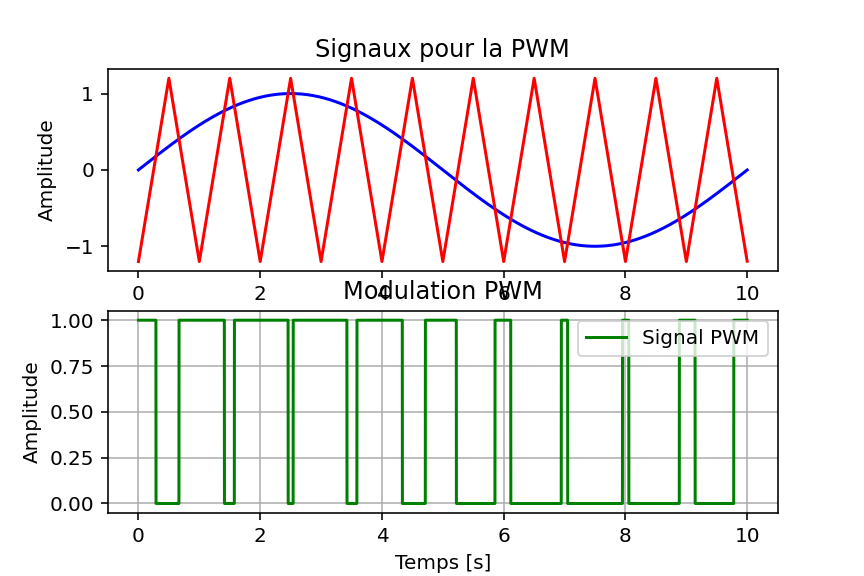
\includegraphics[width=10cm]{images/1.1.1 - PWM btw sin and tri.png}
                \caption{Superposition du signal triangle sur le sinus et modulation PWM correspondante}
                \label{fig:pwm_modulation}
            \end{figure}
            
            Quand on superpose le signal triangle sur le signal sinusoïdale, on peut facilement déterminer la Modulation PWM. En effet, si on y regarde de plus près la superposition des signaux, la modulation est d'amplitude 1 quand le signal triangle passe au dessus du sinusoïdale, et est d'amplitude 0 quand le signal triangle passe en dessus du sinusoïdale. On obtient donc un signal qui alterne entre l'amplitude 1 et 0 en fonction des signaux d'entrée. On peut notamment voir que la modulation a une amplitude de 1 sur des plus grands intervalles de temps aux abords des maxima du sinus, et une amplitude de 0 aux abords des minima du sinus.
        \subsection{Influence de la fréquence du signal triangulaire}
            La fréquence du signal triangulaire utilisé pour la modulation PWM joue un rôle essentiel dans la qualité de la modulation. \textbf{Une fréquence élevée} entraîne une modulation plus fine, ce qui permet de mieux reproduire les variations du signal sinusoïdale. Cela réduit les artefacts de quantification et améliore la fidélité du signal après filtrage. \textbf{Une fréquence trop basse} induit une largeur d'impulsions plus grossière, ce qui introduit davantage de distorsion et rend la reconstitution du signal sinusoïdale plus difficile après filtrage. Cela peut entraîner une perte de détails dans le signal amplifié.
        \subsection{Influence de l'amplitude du signal triangulaire}
            L'amplitude du signal triangulaire influence la largeur des impulsions PWM générées. \textbf{Une amplitude plus grande} que celle du signal sinusoïdale implique que les variations de la largeur des impulsions sont proportionnelles, ce qui garantit une modulation linéaire. \textbf{Une amplitude proche ou inférieure} à celle du signal sinusoïdale peut conduire à une modulation PWM plus déformée, car les impulsions auront une largeur presque constante ou très variable, ce qui perturbera la fidélité de la reconstruction du signal original.
        \subsection{PWM avec $f_{triangle}=20 [kHz]$ et $f_{sinus}=1 [kHz]$}
        \begin{figure}[h!]
                \centering
                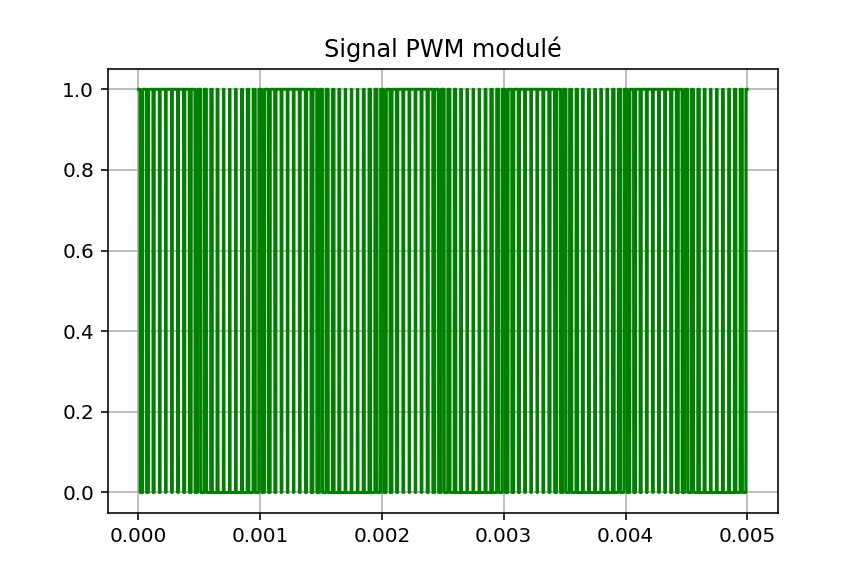
\includegraphics[width=10cm]{images/1.1.4 - PWM btw sin and tri.png}
                \caption{Modulation PWM correspondant à la superposition de l'onde triangulaire et du signal sinusoïdale pour une fréquence d’échantillonnage de $1 [MHz]$}
                \label{fig:echantillon_1MHz}
            \end{figure}
\newpage
        \subsection{Diminution de la fréquence échantillonnage}
            \begin{figure}[h!]
                \centering
                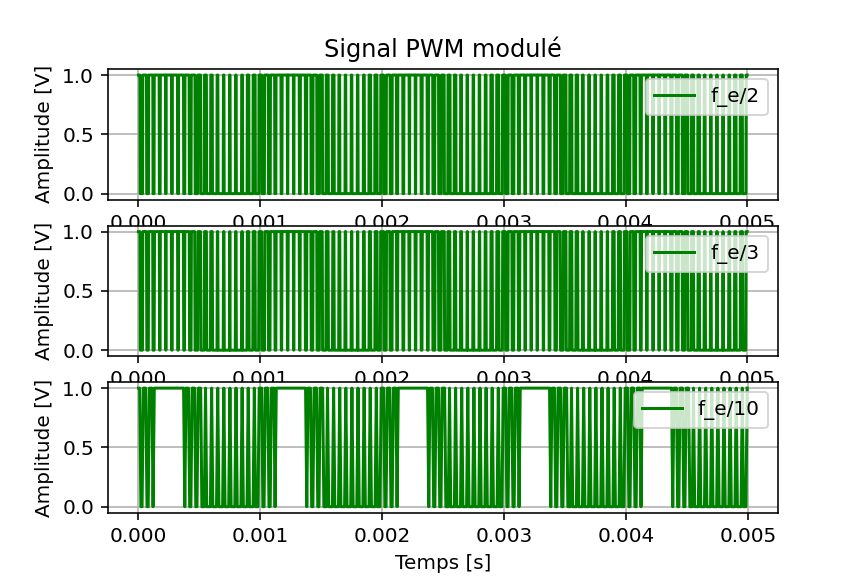
\includegraphics[width=10cm]{images/1.1.5 - PWM btw sin and tri.png}
                \caption{Modulation PWM pour une fréquence d’échantillonnage divisée par 2, 3 et 10}
                \label{fig:comp_freq_echant}
            \end{figure}
            Pour $f_e = \frac{10^6}{10} [Hz]$, le signal PWM se "troue" (intervalles ou le signal est up et sans variation). Ce qui est bien différent du signal que l'on retrouve pour $\frac{f_e}{2}$ et $\frac{f_e}{3}$
        \subsection{Fréquence d’échantillonnage minimale}
            Si l'on se base sur le cours de "Signaux, systèmes et commandes", la fréquence d’échantillonnage doit être au minimum 2 fois supérieure à la fréquence du signal à échantillonner. Cela s'explique que pour un signal sinusoïdale avec une fréquence $f_{sin}$, les maxima et les minima se trouvent à $T = \frac{2}{f_{sin}}$, il faut donc au moins $2f_{sin}$ pour les échantillonner correctement. 
    \section{TDH}
        $TDH = \frac{\sqrt{(\sum |Y_{k.f_0}|^2)-(|Y_{f_0}|^2+|Y_{-f_0}|^2)}}{\sqrt{\sum|Y_{k.f_0}|^2}}<1$
\newpage
    \section{Amplification}
        \subsection{Signal PWM amplifié}
            \begin{figure}[h!]
                \centering
                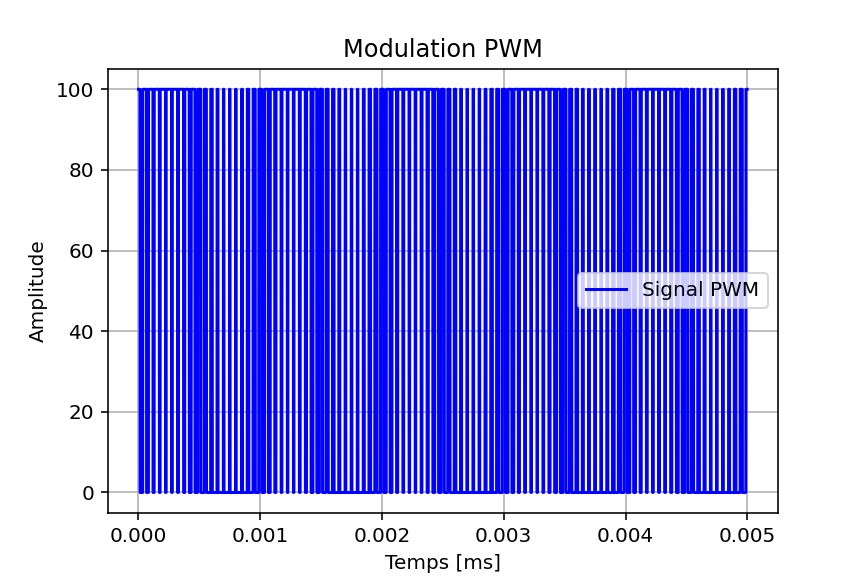
\includegraphics[width = 10cm]{images/1.3.1 - ampl_PWM btw cos and tri.png}
                \caption{Amplification du signal PWM par un facteur 100}
                \label{fig:PWM_amp}
            \end{figure}
\newpage 
        \subsection{Visualisation de \texttt{sc.freqz()} dans Python}
            \begin{figure}[h!]
                \centering
                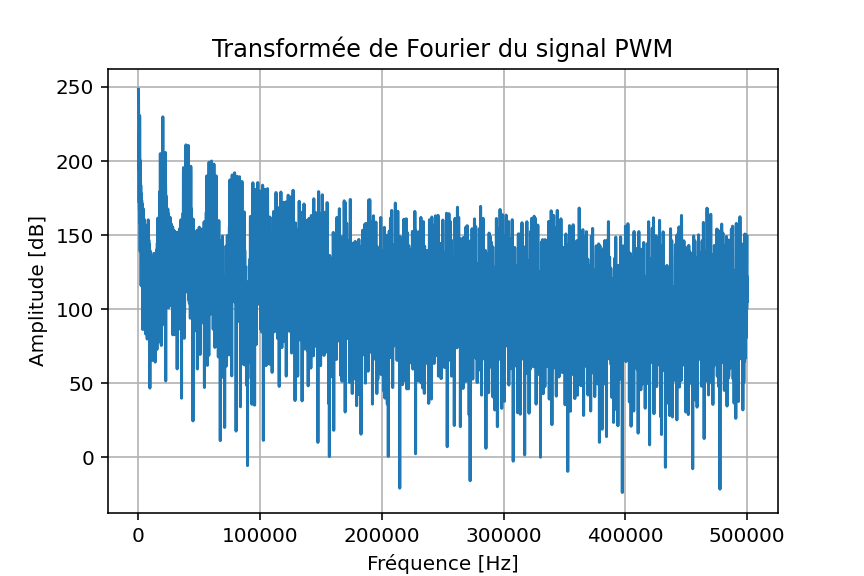
\includegraphics[width = 10cm]{images/1.3.2 - Fourier transform of ampl_PWM.png}
                \caption{Transformée de Fourier du signal PWM après amplification}
                \label{fig:fourier_PWM_amp}
                
                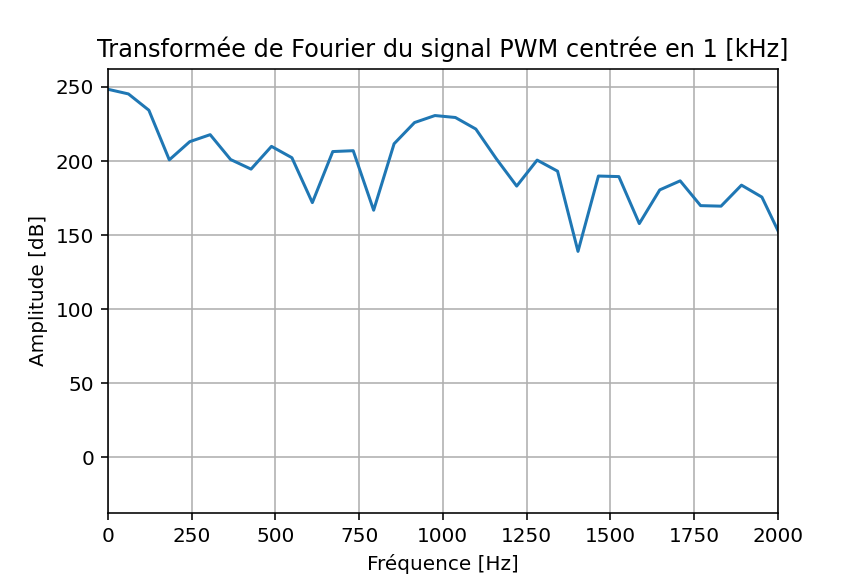
\includegraphics[width = 8cm]{images/1.3.2 - Fourier transform of ampl_PWM centered on 1000 Hz.png}
                \caption{Transformée de Fourier du signal PWM après amplification, centrée en 1 kHz}
                \label{fig:fourier_PWM_amp_1kHz}
                
                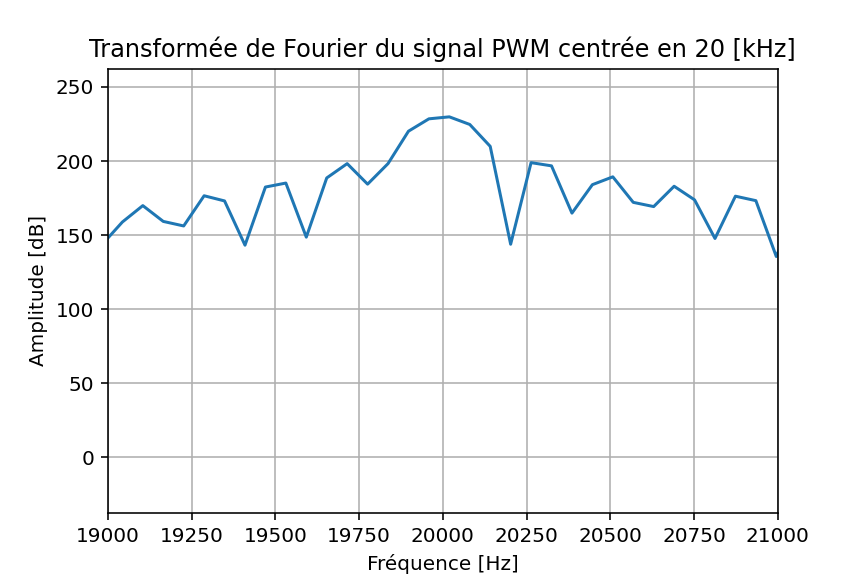
\includegraphics[width = 8cm]{images/1.3.2 - Fourier transform of ampl_PWM centered on 20 000 Hz.png}
                \caption{Transformée de Fourier du signal PWM après amplification, centrée en 20 kHz}
                \label{fig:fourier_PWM_amp_20kHz}
            \end{figure}
        \subsection{Signal de départ}
            Prenons la \hyperref[fig:fourier_PWM_amp_1kHz]{figure 1.6}. Le maximum local que l'on voit représente bien la sinusoïdale de départ. De même avec la \hyperref[fig:fourier_PWM_amp_20kHz]{figure 1.7}, on trouve également un maximum local, correspondant au signal triangulaire. On retrouve donc dans le spectre la fréquence des signaux de départ $f_{sin} = 1[KHz]$ et $f_{triangle} = 20[kHz]$
    \section{Filtrage}
        \subsection{Type de filtre}
            Afin de retrouver la sinusoïde du signal de départ, il faut utiliser un filtre passe bas afin de bloquer toutes les harmoniques issues de la modulation et du signal triangulaire.\\
            \subsubsection{$A_p$ (perte dans la bande passante)}
            Elle détermine combien de perte est acceptable dans la bande passante du filtre. Dans un système audio, on attend typiquement une perte faible. Cela signifie que l'on souhaite que le signal à la fréquence fondamentale passe pratiquement sans atténuation.\\
            \subsubsection{$A_s$ (atténuation dans la bande de coupure)}
            L'atténuation dans la bande de coupure, c'est-à-dire au-delà de la fréquence de coupure, devrait être significative pour éliminer les harmoniques. Cela pourrait être dans la plage de 40 à $60 [dB]$ pour éviter que des composantes indésirables influencent le signal de sortie.\\
            \subsubsection{$\Omega_p$ (fréquence de coupure passante)}
            La fréquence de coupure est déterminée par la fréquence fondamentale du signal sinusoïdal, qui est de $1 [kHz]$. Cette fréquence de coupure peut être légèrement au-dessus de cette valeur, par exemple à $2 [kHz]$ pour s'assurer que la fréquence fondamentale et ses premières harmoniques passent.\\
            \subsubsection{$\Omega_s$ (fréquence de coupure stop-band)}
            La fréquence de coupure dans la bande stop doit être choisie pour éliminer efficacement les harmoniques du signal PWM, qui sont présentes autour de $20 [kHz]$ (la fréquence du signal triangulaire utilisé pour la modulation PWM). 
        \subsection{Evolution du TDH après la modulation}
            La modulation induit des harmoniques autour de la fréquence du signal triangulaire. Cependant cette distorsion cause une perte dans le signal, qui sera visible dans le TDH. C'est là que le filtre intervient et bloque les fréquences harmoniques de la modulation, permettant d'améliorer un peu le TDH. Le TDH augmentera en même temps que la fréquence de la porteuse. 
        \subsection{Ordre de grandeur pour TDH}
            \subsubsection{Avant filtrage} Lors de la modulation PWM, le TDH peut être élevé en raison des nombreuses harmoniques générées par cette modulation. Cependant, après amplification et filtrage, la distorsion due aux harmoniques peut être fortement atténuée.
            \subsubsection{Après filtrage} Le filtrage passe-bas réduit la distorsion des harmoniques au-delà de la fréquence de coupure, et donc le TDH peut descendre à des niveaux entre $0.1[\%]$ et $1[\%]$ (soit une atténuation de $40$ à $60 [dB]$ des harmoniques).
            \subsubsection{Conclusion} Le TDH final pour un amplificateur numérique de classe D, après filtrage, se situera probablement entre $0.1[\%]$ et $1[\%]$, ce qui est un niveau acceptable pour une reproduction sonore de qualité, tout en étant beaucoup plus faible que celui obtenu sans filtrage.
\newpage
\chapter{Conception du filtre de sortie}
    \section{Approximation des filtres}
\newpage
        \subsection{Butterworth}
            Filtre d'ordre 30 avec comme fréquence de coupure $\omega = 0.1615$
            \begin{figure}[h!]
                \centering
                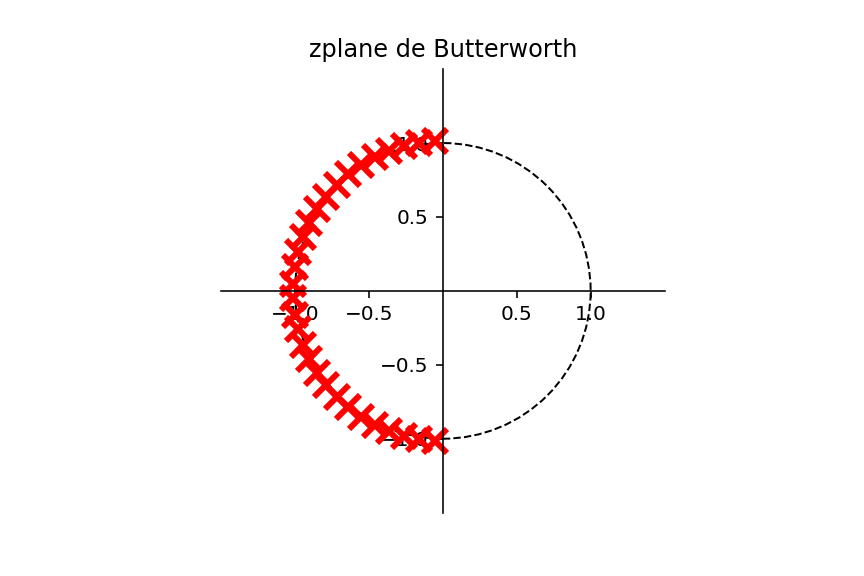
\includegraphics[width = 8cm]{images/2.0.0 - zplane de Butterworth.png}
                \caption{Pôles de l'approximation de Butterworth du filtre}
                \label{fig:zplane-Butterworth}
                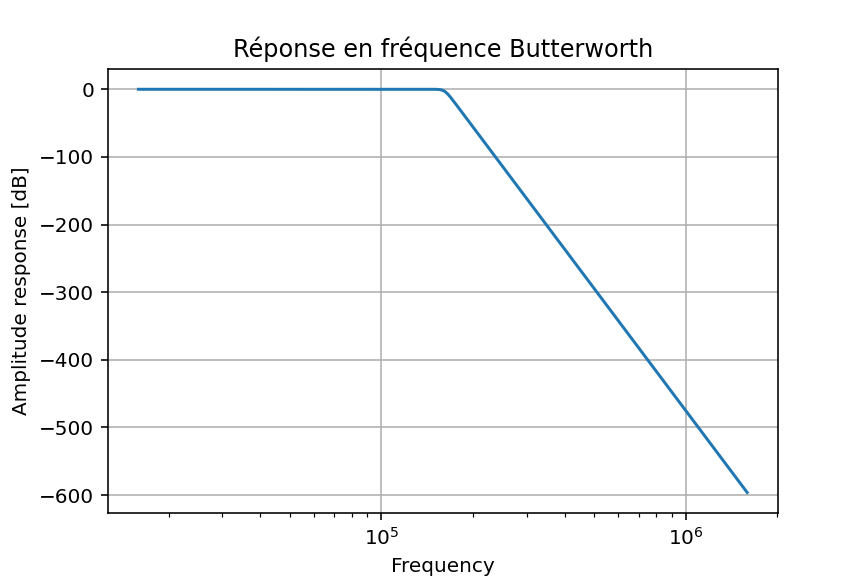
\includegraphics[width = 8cm]{images/2.0.0 - Réponse en fréquence Butterworth.png}
                \caption{Réponse en fréquence de l'approximation de Butterworth}
                \label{fig:repfreq-Butterworth}
            \end{figure}
            
            L'ordre de la fonction de transfert devrait être égal à 5. Or ici, nous avons un approximation d'ordre 30, ce qui dépasse largement l'ordre maximum que nous nous imposons.
\newpage
        \subsection{Chebychev 1}
            Filtre d'ordre 10 avec comme fréquence de coupure $\omega = 0.1592$
            \begin{figure}[h!]
                \centering
                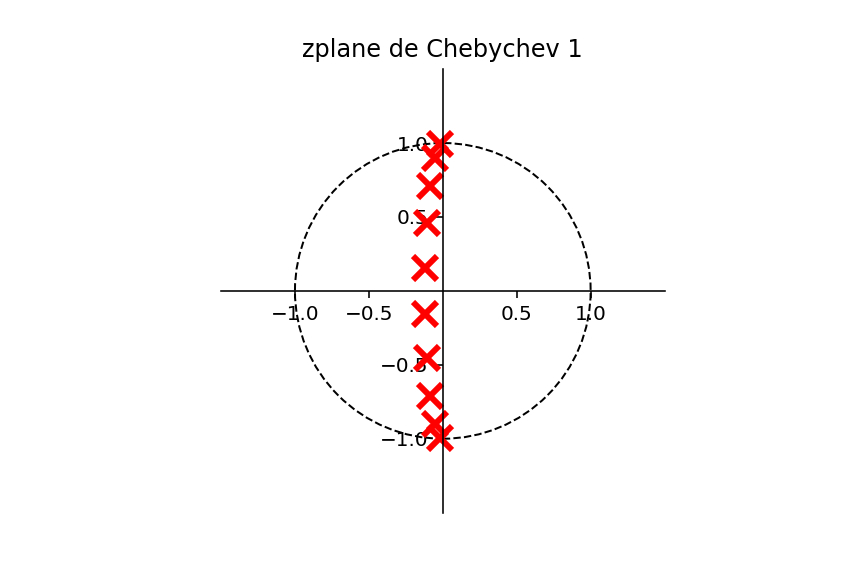
\includegraphics[width = 8cm]{images/2.0.0 - zplane de Chebychev 1.png}
                \caption{Pôles de l'approximation de Chebychev 1 du filtre}
                \label{fig:zplane-Chebychev1}
                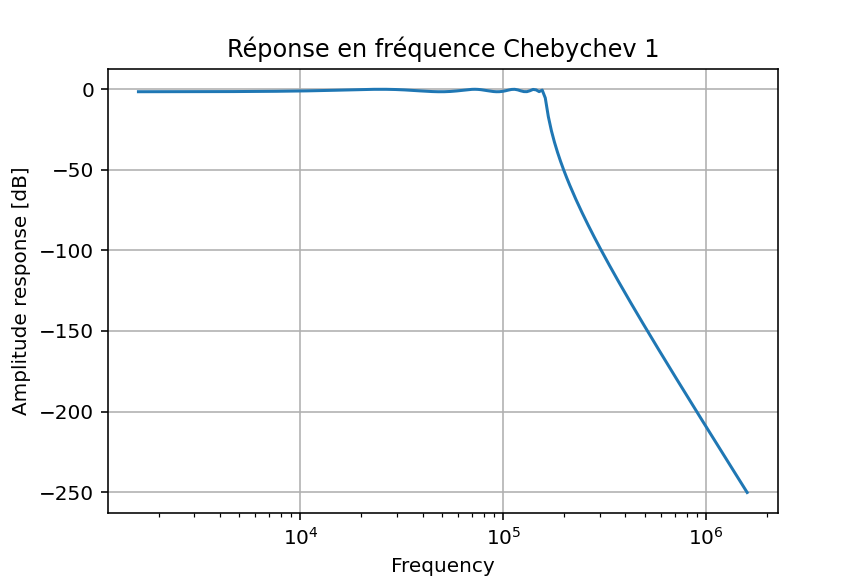
\includegraphics[width = 8cm]{images/2.0.0 - Réponse en fréquence Chebychev 1.png}
                \caption{Réponse en fréquence de l'approximation de Chebychev 1}
                \label{fig:repfreq-Chebychev1}
            \end{figure}
            
            Idem ici, nous avons toujours un ordre supérieur à la tolérance de 5 (la fonction de transfert de l'approximation de Chebychev 1 est d'ordre 10, donc encore trop élevé pour notre étude)
\newpage
        \subsection{Cauer}
            Filtre d'ordre 5 avec comme fréquence de coupure $\omega = 0.1592$ et comme fonction de transfert $H_{Cauer}(p) = \frac{0.047p^4 + 0.22p^2 + 0.23}{p^5 + 0.92p^4 + 1.85p^3 + 1.13p^2 + 0.79p + 0.23}$
            \begin{figure}[h!]
                \centering
                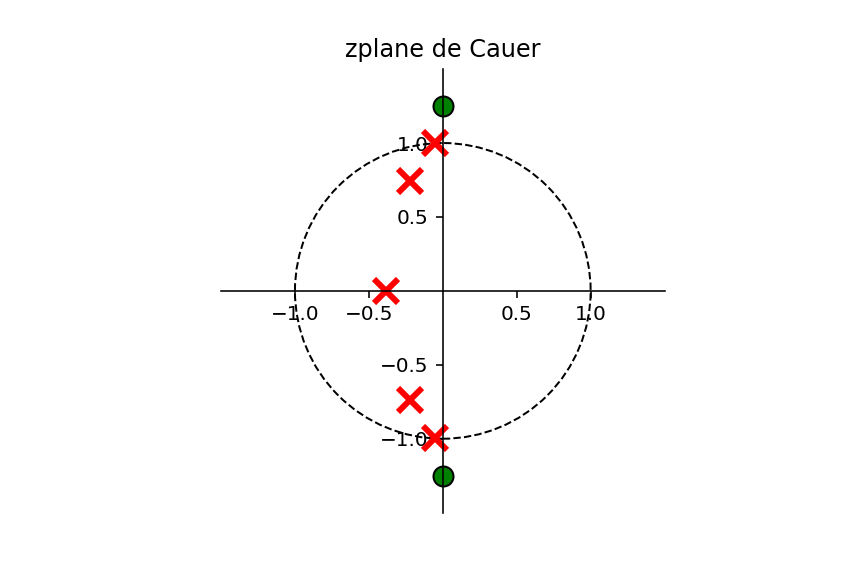
\includegraphics[width = 8cm]{images/2.0.0 - zplane de Cauer.png}
                \caption{Pôles et zéros de l'approximation de Cauer du filtre}
                \label{fig:zplane-Cauer}
                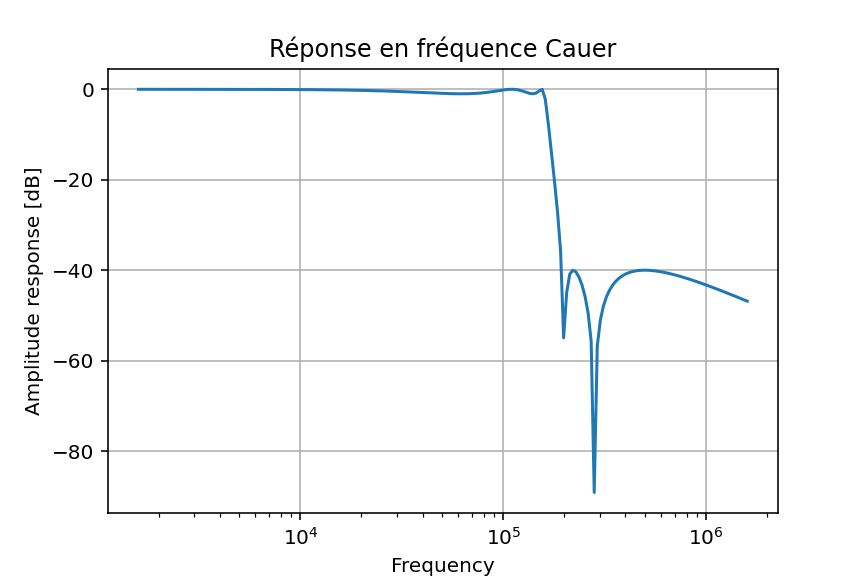
\includegraphics[width = 8cm]{images/2.0.0 - Réponse en fréquence Cauer.png}
                \caption{Réponse en fréquence de l'approximation de Cauer}
                \label{fig:repfreq-Cauer}
            \end{figure}
            
            Pour l’approximation de Cauer, la fonction de transfert est d'ordre 5, elle respecte donc bien notre critère de sélection du filtre passe-bas.
\newpage
    \section{Choix du filtre}
        De par le fait qu'il ne faut pas dépasser un filtre d'ordre 5, seul le filtre de Cauer peut-être considéré ici. 
    \section{Synthèse du filtre}
        Le filtre d'ordre 5 peut être synthétisé à partir des coefficients fournis par la fonction \texttt{sc.ellip()}. Nous devons pour cela utiliser sur les coefficients du dénominateur et du numérateur la fonction \texttt{np.root()} de \texttt{NumPy} pour obtenir les pôles et zéros de la fonction de transfert. Une fois la fonction de transfert obtenue, on peut utiliser la fonction \texttt{np.poly()} afin d'obtenir des coefficients de fractions simples pour les éléments que nous placerons en cascade. \\
        N.B. : Nous approximerons les coefficients des fonctions précédemment calculés dans ce document. A noter que ces derniers ont été implémentés en utilisant toutes les décimales.
        \begin{verbatim}
            # paramètres
            w_min = -2
            w_max = 2

            # calcul des zeros pour les fcts des cellules
            num = np.roots(b)
            den = np.roots(a)
        \end{verbatim}  
        \quad{}Afin d'éviter les surtensions, il faut classer les cellules par ordre croissant de facteur de qualité $Q$. Cela revient à rassembler les pôles et zéros les plus proches afin de minimiser $D = |\rho_{poles} - \rho_{zéros}|$. Ce qui conduit à l’ordre suivant pour nos cellules ; le filtre 3, le filtre 2 et le filtre 1 (nous détaillerons ces filtres dans les points suivants).
        \subsection{Filtre 1}
            \begin{verbatim}
            Input :
            print("num1 = ", np.poly([num[0], num[1]]))
            print("den1 = ", np.poly([den[0], den[1]]))
            print("Gain K_1 =", 20*np.log10(abs(K_1)), "[dB]", K_1)

            Output :
            num1 =  [1.         0.         3.1127137]
            den1 =  [1.         0.09984142 0.99889143]
            Gain K_1 = 9.872417848715616 [dB] =  3.11616820779209
            rho_1 pôles = 0.9977840796453636
            \end{verbatim}
            Le premier filtre aura donc comme fonction de transfert $H_1(p) \approx \frac{p^2 + 3.11}{p^2 + 0.10p + 1}$ avec un correction de gain qui devra être de $\approx -9.87 [dB]$.
        \subsection{Filtre 2}
            \begin{verbatim}
            Input :
            print("num2 = ", np.poly([num[2], num[3]]))
            print("den2 = ", np.poly([den[2], den[3]]))
            print("Gain K_2 =", 20*np.log10(abs(K_2)), "[dB]", K_2)

            Output :
            num2 =  [1.         0.         1.57203342]
            den2 =  [1.         0.43821346 0.59713909]
            Gain K_2 = 8.407725445018915 [dB] =  2.6326084579655618
            rho_2 pôles = 0.35657509331168136
            \end{verbatim}
            Le deuxième filtre aura donc comme fonction de transfert $H_2(p) \approx \frac{p^2 + 1.57}{p^2 + 0.44p + 0.6}$ avec un correction de gain qui devra être de $\approx -8.41 [dB]$.
        \subsection{Filtre 3}
            \begin{verbatim}
            Input :
            print("den3 = ", np.poly([den[4]]))
            print("Gain K_3 =", 20*np.log10(abs(K_3)), "[dB]", K_3)

            Output :
            den3 =  [1.         0.38534434]
            Gain K_3 = 8.283020306162175 [dB] =  2.595081581540222
            \end{verbatim}
            Le troisième filtre aura donc comme fonction de transfert $H_3(p) \approx \frac{1}{p + 0.39}$ avec un correction de gain qui devra être de $\approx -8.28 [dB]$.
\newpage
    \section{Vérification Python}
        \subsection{Cellule 1}
            \begin{figure}[h!]
                \centering
                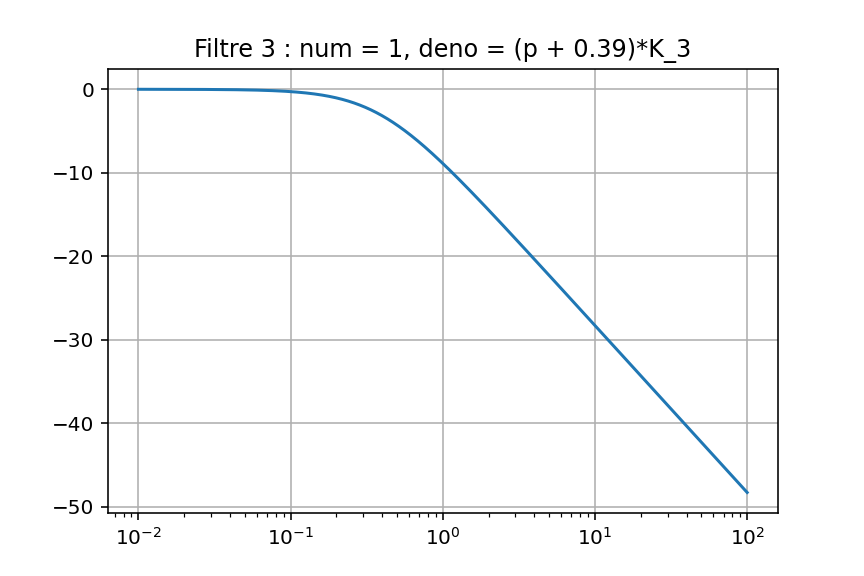
\includegraphics[width = 8cm]{images/2.0.4 - Filtre 3.png}
                \caption{Réponse en fréquence de la première cellule (filtre n° 3)}
                \label{fig:repfreq-filtre-3}
            \end{figure}
            $H_{cell-1}(p)$ est la fonction d'ordre la plus basse parmi les cellules. Pour ce qui est de ses paramètres, il y a un pôle en $\approx \frac{1}{0.39} \approx 2.56$, et notre gain initial vaut $\approx -8.28 [dB]$. Afin de conserver notre gain de Cauer, il est nécessaire de diviser la fonction de transfert $H(p)$ par un facteur $K_3 \approx 2.60$ notre fonction de transfert.
        \subsection{Cellule 2}
            \begin{figure}[h!]
                \centering
                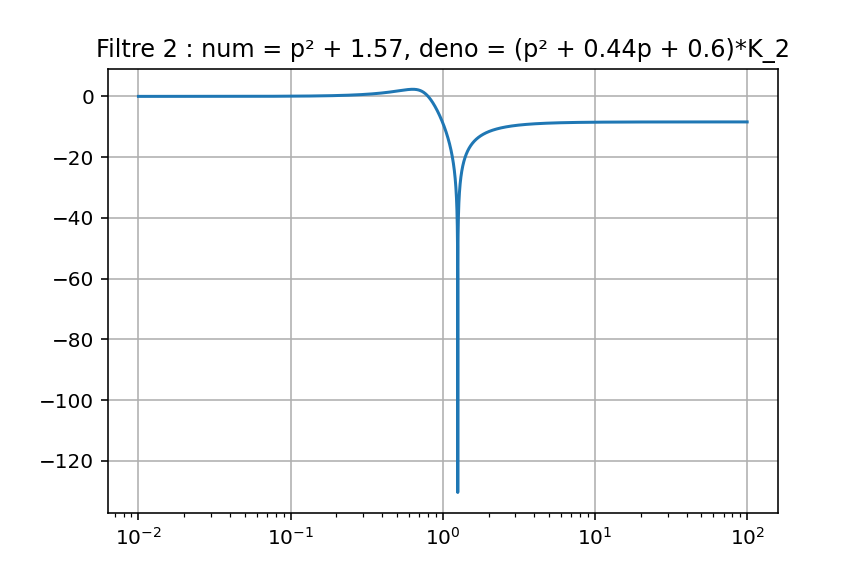
\includegraphics[width = 8cm]{images/2.0.4 - Filtre 2.png}
                \caption{Réponse en fréquence de la deuxième cellule (filtre n° 2)}
                \label{fig:repfreq-filtre-2}
            \end{figure}
            Le facteur $K_2$ vaut $\approx 0.36$, nous devons donc diviser $H_{filtre 2}(p)$ par $\approx 0.36$ pour obtenir $H_{cell-2}(p)$ qui commence bien à $0 [dB]$.
            
\newpage
        \subsection{Cellule 3}
            \begin{figure}[h!]
                \centering
                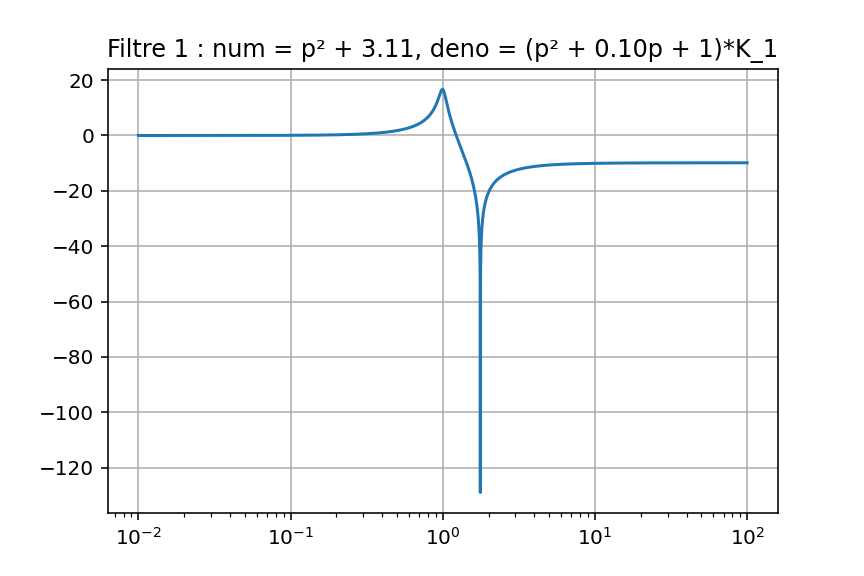
\includegraphics[width = 8cm]{images/2.0.4 - Filtre 1.png}
                \caption{Réponse en fréquence de la troisième cellule (filtre n° 1)}
                \label{fig:repfreq-filtre-1}
            \end{figure}
            Le facteur $K_1$ vaut $\approx 3.12$, nous devons donc diviser $H_{filtre 1}(p)$ par $\approx 3.12$ pour obtenir $H_{cell-3}(p)$ qui commence bien à $0 [dB]$.
        \subsection{Réponse globale}
            \begin{figure}[h!]
                \centering
                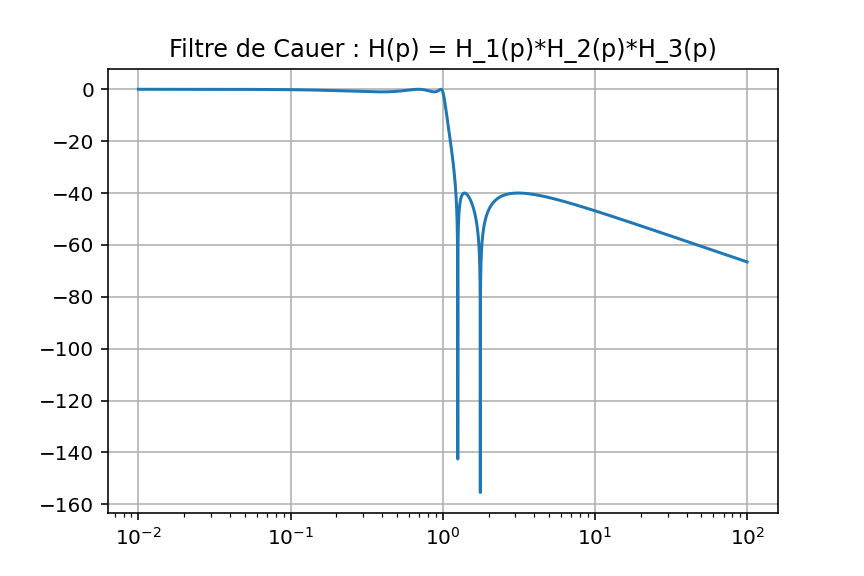
\includegraphics[width = 8cm]{images/2.0.4 - Cauer.png}
                \caption{Réponse en fréquence des cellules mises en cascade}
                \label{fig:repfreq-filtre-1}
            \end{figure}
            On retrouve bien le filtre de Cauer synthétisé au \hyperref[fig:repfreq-Cauer]{point 2.1.3} (à noter que la fréquence de ce graphique n'a pas été dénormalisée et n'est pas affichée avec la même échelle que la figure 2.6). Nous remarquons que le gain pour les basses fréquences vaut bien $0[dB]$ ce qui correspond à un gain $= 1$ sous forme linéaire, nous n'avons donc pas altéré la plage de fréquence qui nous intéresse pour un amplificateur audio (à savoir au moins jusqu'à 20 [kHz], limite de l'audition humaine).
\newpage
    \section*{Conclusion}
        Ce projet a permis d’étudier et de concevoir un amplificateur de classe D en combinant modulation PWM et filtrage pour assurer une qualité sonore optimale. La modulation PWM utilisée repose sur la comparaison d’un signal sinusoïdal ($f_{sin} = 1 [kHz]$) et d’un signal triangulaire ($f_{tri} = 20 [kHz]$, $ A_{tri} = 1.2 [V]$, $ A_{sin} = 1 [V]$). Ces paramètres garantissent une modulation linéaire et réduisent les distorsions. La fréquence d’échantillonnage minimale a été fixée selon le théorème de Shannon pour préserver l’intégrité du signal.\\\\
        Le filtrage a permis d’éliminer les harmoniques générées tout en conservant le signal utile. Parmi les approximations Butterworth, Chebychev 1 et Cauer, le filtre Cauer a été retenu pour répondre à la contrainte d’un filtre d'ordre maximal de 5. Ses paramètres incluent une fréquence de coupure passante supérieure à $20 [kHz]$ et une atténuation en bande stop de $40$ à $60 [dB]$. Le filtre, synthétisé en cascade de trois cellules, optimise les pôles et zéros tout en maintenant un gain constant dans la bande utile.
\end{document}